% \documentclass[sigconf]{acmart}
\documentclass[manuscript]{acmart}
\usepackage{xcolor}
\usepackage{listings}
\usepackage{soul}
\usepackage{xspace}
\soulregister\cite7
\soulregister\ref7

\definecolor{codegreen}{rgb}{0,0.8,0}
\definecolor{codegray}{rgb}{0.5,0.5,0.5}
\definecolor{codepurple}{rgb}{0.58,0,0.82}
\definecolor{backcolour}{rgb}{0.95,0.95,0.92}
\definecolor{grayout}{rgb}{0.5,0.5,0.5}
\definecolor{colgray}{gray}{0.93}
\definecolor{highlightcolor}{rgb}{1,1,0.8}



\newcommand{\grayout}[1]{\textcolor{grayout}{#1}}
\newcommand{\todo}[1]{\textcolor{red}{TODO: #1}}
\newcommand{\question}[1]{\textcolor{codegreen}{Question: #1}}
\newcommand{\eb}[1]{\textcolor{purple}{EB: #1}}
\newcommand{\palani}[1]{\textcolor{codegreen}{PM: #1}}
\newcommand{\leen}[1]{\textcolor{red}{LJ: #1}}

\newcommand{\rom}[1]{\uppercase\expandafter{\romannumeral #1\relax}}
\renewcommand{\labelenumi}{\arabic{enumi}.}
\newcommand{\noofpapers}{\text{124 }}
\newcommand{\primarypapers}{\text{96 }}


\lstdefinestyle{mystyle}{
    %backgroundcolor=\color{backcolour},   
    commentstyle=\color{codegreen},
    keywordstyle=\color{black},
    numberstyle=\tiny\color{codegray},
    stringstyle=\color{codepurple},
    basicstyle=\ttfamily\footnotesize,
    breakatwhitespace=false,         
    breaklines=true,
    lineskip=0.5cm,
    captionpos=b,                    
    keepspaces=true,                 
    numbers=left,                    
    numbersep=5pt,                  
    showspaces=false,                
    showstringspaces=false,
    showtabs=false,                  
    tabsize=2
}

\lstset{style=mystyle}

\newcommand{\mycomment}[1]{}


\def\HiLi{\leavevmode\rlap{\hbox to 0.5\hsize{\color{gray!15}\leaders\hrule height .7\baselineskip depth .5ex\hfill}}}
\def\HiLiS{\leavevmode\rlap{\hbox to 0.05\hsize{\color{gray!15}\leaders\hrule height .7\baselineskip depth .5ex\hfill}}}


\newcommand{\smallblacksquare}{\scalebox{0.6}{$\blacksquare$}}

\AtBeginDocument{%
  \providecommand\BibTeX{{%
    Bib\TeX}}}
\begin{document}

\title{Static Analysis Taxonomies}

\author{Palaniappan Muthuraman}
\authornotemark[1]
\email{palaniappan.muthuraman@upb.de}
\affiliation{%
  \institution{University of Paderborn}
  \city{Paderborn}
  \country{Germany}
}

\begin{abstract}
\textbf{\textit{Context:}}
Static analysis is a fundamental technique in software engineeering used to analyse program code without executing it.
It helps in finding security vulnerabilities, defects in the software system early in the development lifecycle.
Despite its effectiveness, it still faces challenges related to scalability, precision impact, performance overhead, computational complexity.
Traditional static analysis techniques may generate false positives, struggle to scale for large code bases, and demand significant computational resources.
Prior research has demonstrated that the performance of the static analyses can be significantly enhanced through various optimization techniques, such as staging, sparse analysis, and parallelization.\\
\textbf{\textit{Objective:}}
However, these optimizations were implemented as one-off optimizations, applied to a single static analysis in a single analysis context.
Despite the extensive work on static analysis, there remains a lack of a systematic assessment of the various static analysis optimizations techniques,their potential combinations, and the conditions under which combinations are effective. 
The objective is to provide a comprehensive overview of the state-of-the-art static analysis optimizations, examining their individual and joint impact on analysis outcomes.
By analyzing these optimizations both in isolation and in combination, we aim to assess their influence on key performance metrics such as precision, recall, and runtime. 
Furthermore, this study seeks to identify which classes of program benefit most from specific optimizations or combinations of them, thereby offering guidance on the applicability of these optimization techniques in practical analysis scenarios.\\
\textbf{\textit{Method:}}
We conducted a Systematic Literature Review (SLR) by analyzing \noofpapers research papers published in static analysis, program analysis, and software engineering venues over the past 15 years (January 2009 to October 2024).
The primary objective of this review is to gather insights into the problems addressed by these approaches, the fundamental techniques employed, the static analysis sensitivities considered, and the potential for optimization. \\
\textbf{\textit{Result:}}
\todo{Write the results at the end} \\
\textbf{\textit{Conclusion:}}
\todo{Write what has been done and what is been lacking for the futire research to be taken care of}
\end{abstract}

\maketitle
\section{Introduction}
With the introduction of the planned EU Cyber Resilience Act, software developers will soon be required to adopt software assurance techniques to ensure the security and reliability of their software products.
Static analysis is a cornerstone of modern software engineering, examining the code without executing it.
By systematically analysing the code base, static analysis can detect a wide range of security vulnerabilities, bugs, and code smells early in the development process.
This proactive approach not only enhances code quality but also reduces the cost and effort associated with fixing issues later in the software lifecycle.
Static analyses techniques needs to process millions of lines of code, which result in substatial computational overhead.
Moreover, increasing the precision of the analysis - while reducing false positives - typically comes at the cost of longer runtimes and higher resource computation \cite{emanuelsson2008comparative}.
Traditional static analyses approaches often struggle to meet all three objectives simultaneously.

To address these challenges and to improve performance, researchers have proposed numerous optimization techniques, 
For example, a \textbf{staged approach}, where the analysis is divided in successive phases,
each one becoming progressively more precise and computationally expensive \cite{bodden2009verifying,bodden2012partially,jeong2017datadriven,li2018precision,lu2019precision,sinha2010staged,smaragdakis2014introspective}.
The core idea is to include early stages that perform efficient pre-analyses, whose results help avoid unnecessary computations in the later, most costly phases.
\textbf{Sparse Analysis} which restricts computations to only the relevant portions of the program by leveraging value-flow graphs \cite{choi1991automatic,madsen2014sparse,ramalingam2002sparse,spaeth2017ideal}.
While traditional static analyses often operate over the entire program's control flow graph, sparse analysis focuses solely on code segment relevant to the specific analysis at hand, utilizing a value-flow graph composed of the def-use chains.
Prior studies have shown that these optimizations can significanlty enhance performance, reduce analysis time, and in some cases even improve precision. 
However, these optimizations are often implemented as one-off solutions tailored to a specific static analysis and a particular context.

The existing literatute is rich with individual optimization techniques; however, there is a lack of a systematic understanding regarding their compared effectiveness, their potential synergies, and the conditions under which they perform best - whether in isolation or in combination.
When combined, it is crucial to identify which combinations yield the best results, as one optimization can sometimes impede or counteract another.

This study seeks to fill this gap by conducting a \textbf{Systematic Literature Review} of 124 research papers published between Januray 2009 and October 2024 across leading venues in static analysis, program analysis. and software engineering.
Throug this SLR, we aim to:

\begin{enumerate}
    \item Catalog and classify state-of-the-art static analysis optimization techniques.
    \item Examine the interplay between the different optimizations and identify effective combinations.
    \item Determine which classes of programs benefit most from specific optimizations.
\end{enumerate}
\section{Background}
Here comes the background needed for the paper
\section{Methodology for the SLR}
For this SLR, we followed the guidelines provided by Kitchenham \cite{kitchenham2004procedures}

\subsection{Research Questions}

\textbf{RQ1: What are the purpose of these static analysis techniques/optimizations?}
With this research question, we will survey the various optimization techniques in static analysis. \\
\textbf{RQ2: How are the analyses designed and implemented?} \\
In this research question, we conduct a detailed study of the analysis that have been developed. It also includes several sub-questions:\\
\textit{RQ2.1} What fundamental techniques are used for by this static analysis optimization?\\
\textit{RQ2.2} What sensitivity features are applied?\\
\textbf{RQ2: Are the research outputs publcly available?}
We aim to investigate whether the developed tools are open-source or publicly available, reproducible, and easily accessible for use by other practitioners. \\
\textbf{RQ3: What challenges remain to be addressed?}
This question addresses issues that have not yet received significant research attention. It also examines how the focus of the research has evolved over time. 
Additionally, it helps in identifying the research gaps in the current knowledge base, and aims to understand the emerging trends and shifts in priorities within the field.

\subsection{Search Strategy}
This section discusses the keywords we used in our search and the datasets employed to find the relevant publications.

\subsubsection{Search Keywords}
We used the PICOC strategy to develop our search term. Since the \textbf{Intervention (I)} and \textbf{Comparison (C)} terms were not relevant to our scope, they were left empty.

Each of the terms from \textbf{ Population (P)}, \textbf{Outcome (O)}, and \textbf{Context (C)} formed a seperate line in the search string. The final search string was constructed by logically combining these lines, using \textbf{AND} to connect different categories (P, O, C), and \textbf{OR} within each category for synonyms or related terms.
i.e., s =: P \textbf{AND} O \textbf{AND} C \\
Table \ref{tab:picoc_terms} shows the actual keywords we used, which were derived from a manual investigation of relevant publications.

\begin{table}[h]
    \centering
    \begin{tabular}{cc}
    \toprule
    \textbf{PICOC} & \textbf{Search Terms} \\
    \midrule
    P & \text{"control-flow analysis", "data-flow analysis", "static analysis"} \\
    \midrule
    O & \text{"accuracy", "efficiency", "memory usage", "overhead", "performance", "precision", "scalability", "speedup"} \\
    \midrule
    C & \text{"control-flow analysis", "data-flow analysis", "static analysis"} \\
    \bottomrule
    \end{tabular}
    \caption{Search Terms}
    \label{tab:picoc_terms}
\end{table}

\begin{figure}
    \centering
    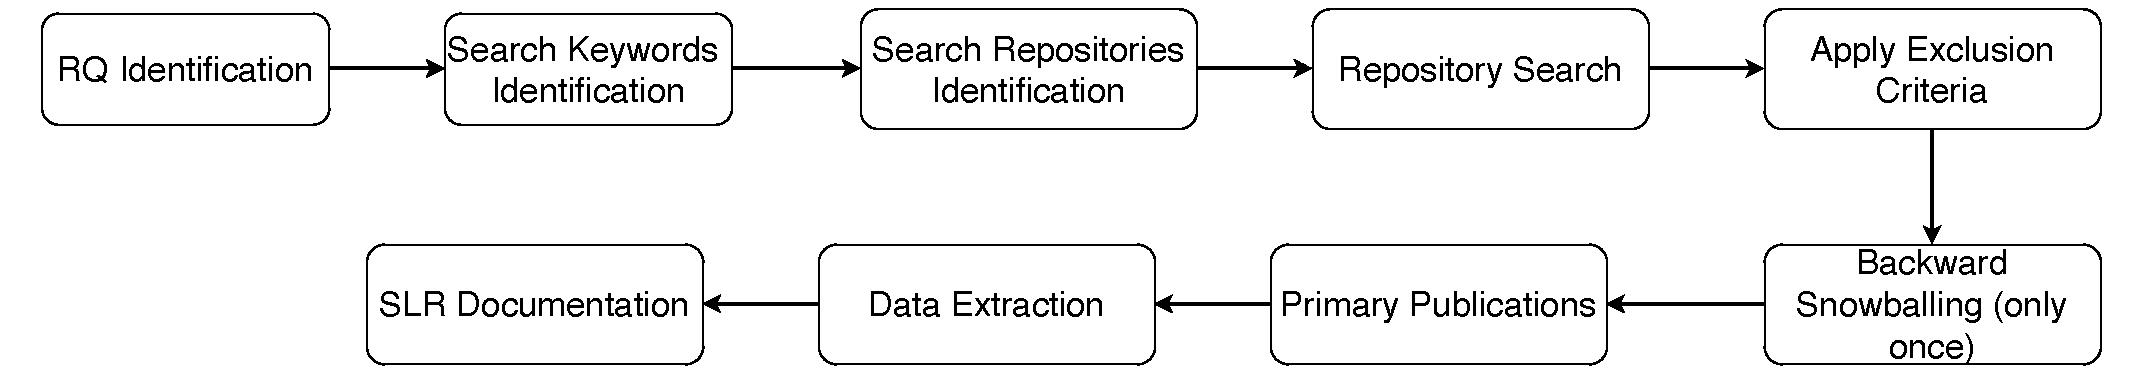
\includegraphics[width=1\linewidth]{figures/SLR.drawio.pdf}
    \caption{An overview of the systematic literature review process.}
    \label{fig:slr-overview}
\end{figure}

\subsubsection{Search Datasets}
We used four well-known repositories, namely ACM Digital Library \footnote[1]{http://dl.acm.org/}, IEEE Xplore Digital Library \footnote[2]{http://ieeexplore.ieee.org/}, Springer Link \footnote[3]{http://link.springer.com/}, and Google Scholar \footnote[4]{https://scholar.google.com/}. Some of these repositories impose restrictions on the amount of search result metadata that can be downloaded. For instance, Google Scholar does not allow frequent search requests from a single device via its API. To overcome this limitation, we used Publish or Perish \footnote[5]{https://harzing.com/resources/publish-or-perish}, a tool that helps retrieve academic documents from Google Scholar. Similarly, Springer Link limits metadata downloads to the first 1,000 search results. However, our search query yielded approximately 10,000 results on this repository. Manually downloading metadata in batches would have been tedious and time-consuming. To handle this efficiently, we used Python scripts to extract data from Springer Link, IEEE Xplore, and ACM Digital Library.

\subsubsection{Exclusion Criteria}
The search terms we used were quite broad, resulting in an exhaustive list of publications. Due to this broad scope, many papers in the search results may be irrelevant to our review. To refine our selection and exclude non-relevant papers, we applied specific exclusion criteria, which are detailed below:

\begin{enumerate}
    \item Given that the majority of scientific publications today are in English, we exclude all non-English papers from our review.
    \item Papers under 5 pages in double-column format or under 7 pages in LNCS single-column format were excluded. Additionally, papers exceeding 30 pages in LNCS single-column format were also excluded.
    \item If multiple papers described the same or similar approaches, we included only the one with the most comprehensive description. For example, an extended journal paper \cite{lu2021eagle} was selected over its shorter conference version \cite{lu2020precision}.
    \item Papers lacking sufficient technical details about their approaches were excluded.
    \item Papers that did not focus on optimizing static analysis itself were excluded. For example, papers that use static analysis to optimize the analyzed program were considered out of scope and excluded.
    \item Papers that focus on dynamic or hybrid analysis were excluded.
\end{enumerate}


\subsubsection{Primary publications selection}
Table \ref{tab:summary_slr} summarizes the results of the search process. For each paper, we first reviewed the title and keywords to determine its relevance to our use case. If the relevance was unclear, we proceeded to read the abstract. If the abstract was still insufficient to make a decision, we skimmed the paper to assess its suitability.
\todo{Usually here we should discuss how many reviewers did read the paper, and how did you overcome the inconsistencies the results?}
In the end, we got \noofpapers papers in total.

\subsubsection{Backward snowballing}
To ensure the completeness of our study and to capture relevant works not identified through our initial search terms, we conducted a lightweight backward snowballing process, performed only once.
The objective was to identify additional papers cited by our initially selected primary publications that align with the scope of our study.
Manual snowballing process it tedious and time consuming, so we developed a series of python scripts to automate and streamline the process.
First, We used pdfx \footnote{https://github.com/metachris/pdfx} to extract the text from the pdf and then retrieved the references from the extracted text.
Subsequently, additional scripts were used to filter out papers which fell outside the defined year boundary of our study scope.
Furthermore, we used python scripts to extract keywords from the paper, and eliminated those that did not align with the scope of our review.
After the automatic filtering stage, we manually reviewed the titles and abstracts of the remaining references. 
Papers found relevant to the scope of study, and not already included in our primary publications set were added to the final list of primary publications.
The relatively high number of additional papers identified through backward snowballing can be attributed to the fine-grained terms used by the original studies, which were not fully covered by our broader search strategy.
For instance, many papers contains keywords such as context-sensitivity, context, parallel processing, call graph, call site sensitivity, which, although highly relevant, were not explicitly included in our original search queries.
Our initial search term aimed for broader coverage, while snowballing allowed us to capture these more granular studies.


\begin{table}
    \begin{tabular}{lccccc}
    \toprule
    Source                         & IEEE & ACM  & Springer & Google Scholar & Total \\
    \midrule
    Search Results                 & 5561 & 3195 & 3980     & 1000           & 13736 \\
    After Reviewing Title/Keywords & 44   & 136  & 13       & 43             & 317   \\
    After Reading Abstracts        & 117  & 30   & 22       & 2              & 171   \\
    After Skimming                 & 72   & 22   & 3        & 20             & 117   \\
    After Final Discussion         &      &      &          &                & 96    \\
    Backward snowballing           &      &      &          &                & 28    \\
    Total                          &      &      &          &                & 124    \\ 
    \bottomrule
    \end{tabular}
    \caption{Summary of the Primary Publications Selection Process}
    \label{tab:summary_slr}
\end{table}
    
\subsection{Pointer Analysis}

Pointer analysis is a fundamental and widely applied static analysis technique that aims to determine the possible objects or memory locations that the pointer variables in a program may reference during execution.
Among the earliest and most influential contributions in this area is the work of Andersen in 1994, known as Andersen's Analysis, which is flow-, context-, and field-insensitive \cite{andersen1994program}. 
This analysis also referred to as a subset based analysis, introduces subset constraints to model the relationships between pointer variables and the memory locations they can potentially point to. 
Following Andersen's work, Steensgaard proposed in 1996 a unification-based pointer analysis that operates with almost linear time complexity \cite{steensgaard1996points}.
Unlike Andersen's approach, Steensgard's analysis merges points-to-set wherever any aliasing between two pointer variables, leading to a coarser approximation of the points-to information. 
As a result, Steensgaard analysis sacrifices precision for scalability, making it significanlty faster and less precise than Andersen's analysis \cite{shapiro1997effects}.
\todo{Should write the difference between context, object, field, flow sensitivity here??.}
\todo{Should write about k-site sensitivity??.}
Since both Andersen's and Steensgaard's analyses are field-, context-, and flow-insensitive, many subsequent researchers sought to improve precision by introducing different forms of sensitivity.
In 1994, Emami et al., \cite{emami1994context} defined a pointer analysis that, while still flow-insensitive, was extended to be context-sensitive. 
Their formulation distinguished between ''may'' and ''must'' points-to relations, thereby enabling strong updates.
Later in 2002, Milanova et al., \cite{milanova2002parameterized} introduced object-sensitive pointer analysis as a novel form of context sensitivity tailored for flow-insensitive points-to-analysis for Java.
Through empirical evaluation, they demonstrated that object-sensitivity provides greater precision than the traditional call-site sensitivity in the context of object-oriented programs.
In 2011, Smaragdakis et al., \cite{smaragdakis2011pick} proposed type sensitivity, a different sensitivity approach that leverages the type information as the distinguishing context.
Subsequently, in 2013, Kastrinis et al., \cite{kastrinis2013hybrid} proposes a hybrid form of context sensitivity that selectively combines both object-sensitivity and call-site sensitivity.
Their experimental research showed that this selection hybrid approach yields higher precision than a naive, non-selective combination of the two sensitivities.

Following the foundational works in pointer analysis, researchers have continually sought to enhance both the precision and efficiency of these analyses.
Starting from 2009, significant strides have been made in optimizing pointer analysis techniques.
In 2009, Lundberg et al., \cite{lundberg2009fast} introduced a context- and flow-sensitive pointer analysis approach that significanlty improves upon traditional methods in terms of both speed and precision.
Their analysis employed a graph-based Static Single Assignment (SSA) form, which extends the conventional SSA form \cite{ssa} to effectively represent points-to information.
In this representation, each method is modeled as a graph where nodes correspond to operations within the method, and edges denote data dependencies between these operations.
By leveraging SSA form, their analysis maintains strict flow-sensitivity.
They also introduced "this-sensitivity". This technique analyses methods seperately for each abstract object reaching the implicit this variable, thereby distinguishing between different calling contexts.
Empirical evaluations demonstrated that their 1-this-sensitivity analysis is considerably faster than the traditional context-sensitive and object-sensitivity analyses.

In 2011, Lhotak et al., \cite{lhotak2011points} proposed a strong update analysis combining best of both worlds: the efficiency of flow-insensitive analysis and the precision of flow-sensitive analysis through strong updates.
The key insight is the use of strong updates which can be applied when the dereferenced points-to set is a singleton. 
In their approach, singleton points-to sets are tracked using a flow-sensitive analysis, while non-singleton points-to sets are handled using a flow-insensitive analysis.
This hybrid strategy allows flow-sensitive analysis to refine the precision of flow-insensitive points-to information, while the flow-insensitive analysis provides a robust fallback in cases where flow-sensitive tracking would be expensive.
The analysis leverages SSA form which is effective to perform strong updates. Empirical results demonstrated that this hybrid method produces more precise points-to sets compared to purely flow-insensitive or purely flow-sensitive approaches.
\section{Incremental}

Traditional data-flow analyses often require recomputation of the entire analysis for every modification in the codebase, regardless of the size or scope of the change.
This approach becomes highly time-consuming when dealing with large codebases.
To address this limitation, researchers have proposed various incremental analysis techniques that efficiently update analysis results in response to code changes, thus avoiding unnecessary recomputation.
\todo{Should talk about reviser updating incrementally for both phases of IDE?}
In 2014, Arzt et al., introduced Reviser, a tool designed to incrementally update IDE-based data-flow analyses \cite{arzt2014reviser}.
Reviser follows a clean-and propagate approach: for each affected node it clears the computed information and recompute the information using all of the node's predecessors.
The algorithm identifies changes in the code and their affected predecessors or successors by computing structural differences between Control Flow Graphs (CFG's).
\todo{Should have this -> Reviser also replaces the standard IDE Solver with one capable of handling incremental updates?}
Experimental results demonstrated that Reviser produces the same results as a full analysis while saving 80\% of time required for a full recomputation.
Notably, Reviser also recomputes the complete call graph.

While Reviser focuses on incremental data-flow analysis in IDE's, In 2017, Sathyanathan et al., \cite{sathyanathan2017incremental} proposed a framework for incremental whole program optimization.
Their framework uses a simple and fast checksum technique to detect changes in the codebase.
Unl;ike Reviser, which targets IDE-based data-flow analyses, this framework is applied directly within the C/C++ compiler.
The primary goal here is to reduce recompilation time rather than update data-flow information

\todo{Add An incremental points-to analysis with CFL-reachability here}

Another important area for incremental pointer analysis is pointer analysis which is central to most interprocedural analyses.
While there has been significant work on parallelizing pointer analysis, relatively little work has focused on making it incremental. \todo{cite}
In 2019, Liu et al., \cite{liu2019rethinking} proposed the first efficient and precise incremental and parallel pointer analysis for Java programs.
This approach detects code modifications by comparing the SSA-based IR of the old and new program.
This algorithm constructs call graphs on the fly and supports efficient parallelelization within each fixed-point iteration.
It leverages a fundamental transitivity property of Andersen's analysis and it is context sensitive, path sensitive, and flow insensitive.
Experimental results shows that this achieves more than 200X speedups over other existing approaches and also 2-5 times faster than the whole program pointer analysis.

Existing techniques typically support either incremental or demand-driven analysis, but not both, and they often impose restrictions such as requiring finite abstract domains.
In 2021, Stein et al., \cite{stein2022demanded} introduced a framework that unifies incremental and demand-driven analysis for any arbitraty abstract domain, even for those with infinite domains and widening operators.
Their approach is based on a data structure called Demanded Abstract Interpretation Graph (DAIG), which treats program edits, client queries uniformly.
By capturing dependencies between statements, abstract states, and intermediate computations, DAIG enables efficient reuse of previously computed results while preserving soundness.


Most recently, In 2024, Krishna et al., \cite{krishna2024fly} developed a dynamic algorithm for handling the addition and deletion of lines in the source code with a guarantee that each such modification takes
linear time in the worst case. Every edge insertion can be handled by reusing the already constructed component graph, 
while deletions- which typically requires global re-evaluation of the entire graph - are optimized using techniques from dynamic undirected connectivity and sparsification.
Although, construction of the initial component graph requires $O(n^2)$ time due to dense graph, subsequent updates can start from a preliminary component graph.

These analyses optimize different aspects of incremental computation, and many of them can be complementary when combined - for example, 
pairing parallel fixed-point computation with dynamic graph updates can further improve efficiency. At the same time, paralelization must be integrated with care, as it can interfere with determinstic guarantees required by incremental solvers.








\subsection{Taint Analysis}

The Interprocedural Finite Distributive Subset (IFDS) problem is a fixed-point, flow- and context-sensitive data flow analysis problem. 
In IFDS, data flow is reduced to a reachability problem over the exploded supergraph. The IFDS algorithm is both memory- and compute-intensive, with a worst-case complexity of
$O(|E| . |D|^2)$ in space and $O(|E| . |D|^3)$ in time where E denotes the number of edges in the supergraph and D denotes the set of data flow facts in the program \cite{reps1995precise}.

A prominent application of the IFDS framework is taint analysis, which tracks the flow of sensitive data through programs.

In 2014, Arzt et al. introduced FlowDroid \cite{arzt2014flowdroid}, a precise, context-, flow-, field-, and object-sensitive static taint analysis tool for Android applications. FlowDroid constructs an interprocedural control-flow graph and leverages the IFDS framework to propagate taints efficiently. 
While FlowDroid remains a state-of-the-art tool widely used in research and security analysis, it has been reported to suffer from poor scalability: 
analyzing large Android applications consumes excessive memory and time due to its precise sensitivities. \cite{li2021scaling}

In 2017, Grech et al., proposed PTaint \cite{grech2017p}, showing that existing points-to analysis implementations can be reused—almost without modification—to compute information flow, thereby unifying points-to and information-flow analysis. 
However, PTaint is flow-insensitive, which may introduces false positives.

Since IFDS solvers typically require substantial memory—sometimes exceeding 100 GB of RAM—several works have sought to improve scalability \cite{li2021scaling}:

In 2019, Choi et al., \cite{choi2019scalable} introduced STAR, a taint analysis tool that is both context- and flow-sensitive and supports multi-source taint analysis.
STAR employs a novel summarization technique called as Symbolic Summarization, which replaces concrete taint sources with symbolic taint sources.
The authors argur that many temporary objects are local to their allocation sites, do not escape, and therefore need not be propagated beyond their allocation sites.
To improve scalability in the IFDS analysis, STAR applies three state-pruning techniques such as escape-based pruning \cite{choi1999escape}, access-based localization \cite{oh2011access}, and bypassing \cite{oh2011access}.

In 2019, He et al., \cite{he2019performance} proposed SparseIFDS, a sparse alternative to traditional IFDS. 
Instead of pre-constructing full control-flow graphs, SparseDroid constructs sparse control-flow graphs on demand for each data flow fact, allowing direct propagation to relevant use sites. 
This approach reduces overhead and achieves an average 22× speedup over FlowDroid while also lowering memory usage when evaluating with the FossDroid dataset \cite{fossdroid}.

In 2021, Li et al., \cite{li2021scaling} introduced DiskDroid, A disk-assisted IFDS solver that reduces memory requirements. 
Instead of storing all path edges, DiskDroid memorizes only frequently accessed (“hot”) edges using a Hot Edge Selector. 
Non-hot edges are recomputed on demand, and inactive edges are swapped to disk once memory usage crosses a threshold. 
This optimization allows DiskDroid to analyze Android apps with only 10 GB of memory, compared to the 128 GB required by FlowDroid, while incurring only a modest overhead, when evaluated with F-Droid \cite{fossdroid}.

In 2021, Arzt et al., \cite{arzt2021sustainable} introduced CleanDroid, An efficient, method-level garbage collector for IFDS solvers. 
CleanDroid reclaims memory by discarding intermediate data flow facts (edges and taint abstractions) that are no longer needed. 
Integrated into FlowDroid, CleanDroid reduces memory consumption by 63\% on average without sacrificing precision. 
However, its method-level granularity is conservative, leaving many non-live edges uncollected and occasionally requiring reprocessing of previously collected edges.

In 2023, He et al., \cite{he2023reducing} developed Fine-Grained Path Edge Collection, to address CleanDroid’s limitations, They proposed a data-fact-level garbage collection algorithm (FPC). 
Unlike CleanDroid, which operates at the method level, FPC selectively collects non-live path edges at a finer granularity, reducing both memory consumption and analysis time. On average, FPC outperforms CleanDroid by a factor of 1.7× in runtime.

In 2023, Gui et al., \cite{gui2023merge} introduced MergeDroid which targeted at reducing redundant computation in IFDS analyses. 
Traditional IFDS repeatedly propagates equivalent value flows, and its context-insensitive activation statements lead to false positives. 
MergeDroid merges equivalent value flows linked to the same abstraction, eliminating redundancy and improving precision. It demonstrates an average 9× performance improvement compared to traditional approaches.

In 2024, Li et al., \cite{li2024boosting} proposed IDEDroid, a novel approach for field-sensitive data flow analysis within the IFDS/IDE framework. 
Traditional field sensitivity requires the use of access paths, which generate a large number of data flow facts and hinder scalability. 
IDEDroid reinterprets access-path generation as a context-free language (CFL) problem, encoded as an IDE problem, thereby allowing propagation only of the base variable. 
This substantially reduces the number of facts generated and improves scalability.

In 2024, Li et al., \cite{li2024boostingmultisolver} introduced SADroid, a tool with flow-sensitivity optimizations. 
Flowdroid relies on the concept of an activation unit, which marks the source location where the data-flow becomes active.
However, each data-flow fact is cloned multiple times at different activation points leading to substantial increase in the number of data-flow facts.
While activation units enable flow-sensitivity, they also causes significant overhead in both runtime and memory usage, with number of data-flow facts growing by up to 9.55x.
To address this, SADroid simplifies the data-flow fact by disregarding activation points and uses a flow-sensitive path builder, which searches for taint propagation paths in a flow- and context-sensitive manner.


\todo{This text talks about the tool as a whole}
When considering which optimizations can be combined, pairing SparseDroid with garbage collection approaches (CleanDroid or FPC) is unnecessary. 
SparseDroid’s sparse control-flow graph already ensures that only live edges are present, so adding GC would introduce computational overhead without yielding additional efficiency gains. 
Similarly, combining SparseDroid with DiskDroid is redundant, since SparseDroid already incorporates a caching mechanism for sparse CFGs. 
On the other hand, SparseDroid and MergeDroid complement each other well: SparseDroid reduces the number of propagation paths, while MergeDroid eliminates redundancy within the propagated facts.

\todo{This talks just about the optimizations that can be combined}
\todo{Which one can be added in the final draft?}
While each optimization addresses specific limitations of IFDS-based taint analysis, these techniques are not mutually exclusive.
For example, disk-assisted storage could be combined with method-level garbage collection to simultaneously lower memory usage and avoid costly recomputation of discarded states.
Similarly, sparse graph construction could be integrated with flow-sensitive path building to minimize number of edges explored.
However, not all optimizations are naturally compatible, and some may undermine each other's effectiveness. 
For example, fine-grained garbage collection and disk-assisted storage both manage memory reduction, but combining them could introduce execessive overhead.
Likewise, symbolic summarization, which abstract taint sources, may conflict with flow-sensitive path building, as the loss of concrete allocation details, can diminish the precision needed for fine-grained flow tracking. 
\section{Graphs}
Understanding how control flows through the program, how data moves between the variables, and how different program components
depend on each other is a very crucial thing to know before any analysis.

There are 4 different widely used graph structures for them namely Control Flow Graph (CFG), Value Flow Graph (VFG), Program Dependence Graph (PDG), and System Dependence Graph (SDG)

Graphs

- Flow-sensitive, context-sensitive, and object-sensitive information flow control based on program dependence graphs (Hammer et al., 2009):
The Information Flow Control (IFC) is used to analyze a program for security leaks. Existing approaches are not precise enough, that means they report too many false alarms. Therefore in this paper 
they use program dependence graphs (PDG) for Java bytecode to implement IFC. Their approach is more precise and it is flow-, context and object-sensitive. One limit of their approach is that 
they can only deal with medium-sized programs (up to 100kLOC).

-  Speeding up context-, object- and field-sensitive SDG generation (Graf, 2010):  In their presented approach they generate SDGs (System dependence graph) efficiently for Java. It is context-, 
field- and object-sensitive and is based on the WALA framework. They showed that their approach reduces time and memory and can improve precision. The technqical background is that the size of object trees 
can become large if the points-to analysis is less precise, so they can't be used in SDGs. In their paper they introduce object graphs, an extension of object tress. As a result they merge duplicate information 
to save space. 

-  Quantitative Interprocedural Analysis (Chatterjee et al., 2015):  They present an efficient algorithm which can answer several static analysis questions, e.g. estimating the average energy consumption (cite).
For that they need the ICFG and a positive weight function which determines for every transition a positive number which says how good, bad or neutral this transition (event) is. 
After that their algorithm compares the good and bad events and determine whether a given threshold is reached in a run. As a result they can quantify the ICFG. Their algorithm is implemented in the Java soot framework 
and can deal with recursion and is sound. But one limit is that they have not consider mulitple quantitative objectives yet but are aiming that in the future. (TODO: have they already done that and can we find improvements?)

-  A Precise Framework for Source-Level Control-Flow Analysis (Riouak et al., 2021):  Their presented framework is called INTRACFG which constructs precise intraprocedrual CFGs. It is based on reference 
attribute grammers and enables the construction of CFGs which are independent of the shape and structure of the AST because other frameworks for constructing CFGs are usually depending from the structure of ASTs. 
INTRACFG only connects AST nodes of interest in the CFG. Attribute grammers denote AST nodes with attributes, reference attribute grammers extend them: their values are references to other AST nodes (cite). 
In their work they achieved to reduce the number of nodes and edges in the CFGs by over 30% compares to other framework. 

-  Efficient Path-Sensitive Data-Dependence Analysis (Yao et al., 2021):  They present a path- and context-sensitive data-dependence analysis with the goal to solve the  aliasing-path-explosion problem 
via a sparse and demand-driven approach. The exisiting challenge for data-dependence analysis is the aliasing-path-explosion problem which means to tracks a large amount of aliases. Their approach summarizes 
data dependence as symbolic and storeless value-flow graphs and they perform a demand-driven phase that resolves transitive data dependence over the graphs. The presented framework is called FALCON, a fused and 
sparse approach for path-sensitive data-dependence analysis. First their approach computes storeless value-flow graphs, as a result no duplicated edges. Then this graph is used for data-dependencies in a 
demand-driven way. By that a path- and context-sensitive def-use information is tracked on demand. It is more efficient because the data dependency can be figured out without points-to information 

-  Path-Sensitive Sparse Analysis without Path Conditions (Shi et al., 2021) :  The sparse program analysis considers only necessary control flows but is still expensive for path-sensitive analysis (cite). 
In this work the authors present Fusion, a fused approach to inter-procedurally path-sensitive sparse analysis (cite). They can determine the path feasiblity without knowing the path conditions, 
this saves cost and time. In their approach the SMT solver works on the program data dependece graph. That's how they can determine path feasibility directly.
They showed that they were able to detect a lot of bugs in mature open-source software with their approach,faster than two other state-of-art approaches. Fusion can analyze milliones of lines of code within a 
short time and less memory compared to other approaches. They achieved the precision of inter-procedural path-sensitivity.

\section{Call Graphs}
In 2016, Petrashko et al., introduced context-sensitive call graph construction algorithms that leverage generic type information in object-oriented languages. 
They proposed two extensions to Scala: one that uses actual type arguments for method contexts and another that refines contexts using more precise subtypes from static types of actual arguments. Their approach significantly improved call graph precision and reduced analysis time, demonstrating the value of incorporating generic type information into call graph analyses.

In 2020, Santos et al., introduced Salsa targets Java programs with serialization and deserialization, enhancing existing points-to and call-graph analyses. It employs an on-the-fly, iterative framework that refines call graphs under explicit assumptions about serialization-related behavior. It addresses the challenges of performing static analysis on programs with dynamic features, particularly focusing on serialization and deserialization processes. To regain soundness, Salsa injects synthetic nodes and edges modeling serialization effects into previously computed call graphs and re-analyzes until convergence. Initial results on the Java Call Graph Test Suite (JCG) indicate that Salsa improves call-graph soundness for programs exercising serialization features.

In 2022, Le-Cong et al., introduced AutoPruner, a novel technique for call graph pruning that utilizes both statistical semantic and structural analysis to eliminate false positives in call graphs. Unlike previous machine learning approaches that primarily relied on structural features, AutoPruner employs a Transformer-based model to capture semantic relationships between caller and callee functions. Unlike cgPruner and pure program-analysis methods that consider only the caller, AutoPruner analyzes the source code of both the caller and callee for each edge. It derives semantic embeddings using a pre-trained code model (e.g., CodeBERT), which can learn relationships from paired inputs, and combines them with per-edge structural features. Given a call graph from a static analyzer, AutoPruner preprocesses the graph, extracts these features, and feeds them to a neural classifier that predicts false-positive edges; predicted false positives are pruned to yield a more precise call graph with fewer false alarms.
Empirical evaluations demonstrate that AutoPruner significantly outperforms state-of-the-art methods, achieving up to 13\% improvement in F-measure and reducing false alarm rates in client analyses.

In 2024, Santos et al., introduced Seneca, a call-graph construction technique for Java that makes serialization and deserialization callbacks explicit. By combining taint analysis with API modeling, it resolves callback targets arising during (de-)serialization to produce sound call graphs with minimal overhead. Seneca performs a novel taint-based call graph construction, which relies on the taint state of variables when computing possible dispatches for callback methods.  In evaluation, Seneca identifies vulnerable paths related to untrusted deserialization, passes all serialization-callback tests, and yields fewer spurious edges than Soot and OPAL, while remaining practical in performance.

In 2024, Helm et al., introduced Unimocg, a modular call-graph framework that separates type-information computation from call resolution, enabling interchangeable algorithms and language-feature modules. It supports reuse of type information in downstream analyses, preserves soundness across ten algorithms without precision or performance loss, and outperforms Soot and WALA's emulated RTA.


\todo{Future Directions and Combinations}

Future work should investigate composing modular construction and pruning techniques to further improve efficiency and precision. A practical pipeline could construct call graphs with Unimocg and subsequently prunes edges with AutoPruner. Seneca can also be integrated as the serialization/callback module within Unimocg, followed by AutoPruner to remove residual false positives. 
As an alternative, Salsa's serialization modeling can precede AutoPruner. For Scala codebases, Petrashko et al.'s context-sensitive construction can be paired with AutoPruner. Seneca and Salsa should not be combined in the same pipeline because they target the same (de-)serialization callbacks; one should be selected based on requirements.


\bibliographystyle{ACM-Reference-Format}
\bibliography{bibliography}

\end{document}
\endinput
